\section{Performances of the Algorithms}
We want now to focus our attention on the performances reached by our implementations of the LZ77 and LZSS algorithms in relation both with the type of file we are trying to compress and the parameters setting, that is the lengths of the \textit{searching window} and the \textit{coding window}.

\subsection{Testing files}
All the experiments we performed have been executed on seven specific types of files, part of them taken from the \textit{Canterbury Corpus}, a collection of files with several formats to be used as sample files for compression testing. The used files are here reported:

\begin{itemize}
\item
\textbf{\texttt{rep.txt}}: simple text file containing a sequence of character \texttt{A} repeated $10000$ times ($10000$ bytes);

\item
\textbf{\texttt{per}}: file containing $10$ repetitions of a random sequence of $1000$ bytes ($10000$ bytes);

\item
\textbf{\texttt{ran}}: file generated by concatening $10000$ random bytes ($10000$ bytes);

\item
\textbf{\texttt{shak.txt}}: simple text file reporting a piece of a Shakespeare poem ($13741$ bytes);

\item
\textbf{\texttt{web.html}}: html format page ($24603$ bytes);

\item
\textbf{\texttt{code.c}}: piece of \texttt{c} code ($11150$ bytes);

\item
\textbf{\texttt{sum}}: SPARC executable file ($38240$ bytes).
\end{itemize}

We chose these files to have a wide span among different kinds of files and show, in this way, the several behaviours the algorithm can assume for different scenarios. In particular, we use the file \texttt{rep.txt} to obtain the maximum compression capability of the algorithm, the file \texttt{per} was included to show the behaviours in presence of periodicity and the file \texttt{ran} represents the worst scenario for compression purposes, since it has no redundancy to exploit and a high entropy. The last four files, on the other hand, do not represent borderline or special cases, but more common examples of files one can deals with during his ordinary life. in the next sections we will see how the algorithms behave working with each of these files.

\subsection{Redundant file}
The first file, \texttt{rep.txt}, is the most redundant file we can have: $10000$ repetitions of the same character, \texttt{A}. The nature of the file allows a very strong compression, since we could just say what is the symbol and how many times it is repeated. The following table shows the performances of the algorithms executed with a fixed \textit{coding window} of length $2000$ and a \textit{searching window} varying between $1000$, $5000$ and $10000$, which is the length of the message itself:
\begin{center}
\begin{tabular}{r | c | c |}
\multicolumn{3}{c |}{\texttt{rep.txt}} \\ \hline
$L_s$ & LZ77 & LZSS \\ \hline
1000 & $0.25$\% & $0.19$\% \\
5000& $0.27$\% & $0.20$\% \\
10000& $0.28$\% & $0.21$\% \\
\hline
\end{tabular}
\end{center}

As we expected the compression is very high: we can represent $10000$ bytes with less than $30$ bytes. It may look strange that performances drop with the increasing of the \textit{searching window}; this is due to the number of bits we need to encode a triplet, which raises with the length of the window (in LZ77 we use $29$ bits when $L_s = 1000$, $32$ bits when $L_s = 5000$ and $35$ bits when $L_s = 1000$). LZSS works to solve this issue, as a matter of fact it behaves slightly better than LZ77 and manages to encode the dictionary with less bits. In this case we can see that the length of the \textit{coding window} has also a great relevance on performances; the followig table summarizes the results obtained when we use the same three searching lengths of the previous example, but a coding length $L_c = 10000$:
\begin{center}
\begin{tabular}{r | c | c |}
\multicolumn{3}{c |}{\texttt{rep.txt}} \\ \hline
$L_s$ & LZ77 & LZSS \\ \hline
1000 & $0.11$\% & $0.08$\% \\
5000& $0.22$\% & $0.08$\% \\
10000& $0.12$\% & $0.09$\% \\
\hline
\end{tabular}
\end{center}
In this case we just need about ten bytes to represent the whole message and the dictionary is composed by only two rows.
It is interesting to report here the 3D plot of the LZ77 performances, in percentage of compression, in function of $L_s$ and $L_c$:

\begin{center}
\begin{figure}[H]
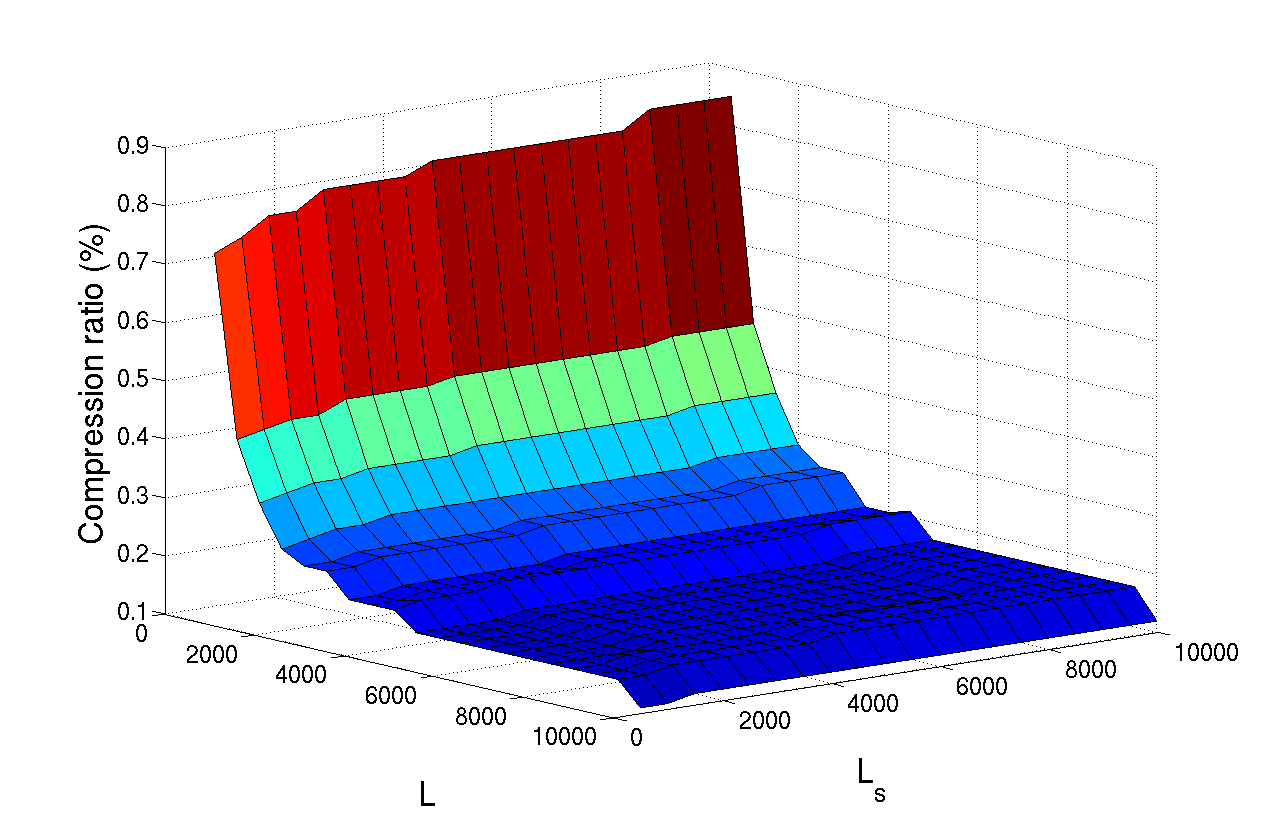
\includegraphics[width=8.5cm]{images/rep_surf.png}
\caption{LZ77 compression ratio in function of $L_s$ and $L_c$.}
\end{figure}
\end{center}

\subsection{Periodic file}
A big problem with implicit dictionary based compression algorithms is that periodicity of the message could not be properly exploited. This unfavorable event occurs if the windows are shorter than the period of the message, such that there is no way the algorithm can become aware of the existance of periodicity in the message. We can bring a clear example compressing the file \texttt{per} keeping fixed the \textit{coding window} to $2000$, but with two different \textit{searching window} lengths: $500$ (half a period) and $5000$ (five times a period). The compression results are reported in the following table:

\begin{center}
\begin{tabular}{r | c | c |}
\multicolumn{3}{c |}{\texttt{per}} \\ \hline
$L_s$ & LZ77 & LZSS \\ \hline
500 & $189.98$\% & $112.53$\% \\
5000& $23.55$\% & $11.44$\% \\
\hline
\end{tabular}
\end{center}

It is clear that, in the first case, the algorithm is not exploiting the periodicity, in fact it is expanding the data and increasing the file dimension, because, being the period built randomly, it finds no redundancy to exploit. In the second scenario, however, periodicity is exploited and the file is strongly compressed.

\subsection{Randomly generated file}
When a file is made by a random sequence of bytes its entropy is very high and the algorithm finds no redundancy to exploit for compression. In this case performances are very low, in fact the output file has a greater dimension than the input file and we can do very little also by varying $L_s$ and $L_c$. The following table reports the compression ratios with $L_c = 2000$ and $L_s = 1000, \ 5000, \ 10000$:

\begin{center}
\begin{tabular}{r | c | c |}
\multicolumn{3}{c |}{\texttt{ran}} \\ \hline
$L_s$ & LZ77 & LZSS \\ \hline
1000 & $184.66$\% & $112.53$\% \\
5000& $197.83$\% & $112.55$\% \\
10000& $202.12$\% & $112.56$\% \\
\hline
\end{tabular}
\end{center}

We can notice two main facts: the first is that LZSS compresses in general better than LZ77; the second is that LZSS' performances decrease much more slowly than LZ77's; if we inspect the dictionaries created by the two algorithms, we can try to spot the reason of such difference: the LZ77 dictionary contains a lot of references to an only previous symbol and we cannot avoid using a whole triplet to encode them. On the other hand the LZSS algorithm is able to realize that it is not a good deal to waste a whole triplet to express an only symbol and it encodes it as a single byte. In this way we ideally would have a dictionary with the same dimensions of the message, but, unlucklily, the coding algorithm also includes the flag bits. Thus, it is practically quite impossible to compress a random sequence: if we try to compress it, we are going to hopelessly expand it.

\subsection{Common files}
The file \texttt{shak.txt} is an example of humanly-written text file. As we can see from the results of the experiment, LZ77 and LZSS are not the best choice for compressing this kind of file. The reason is that the spoken language has not a strong redundancy and patterns of characters are often short and repeated only a few times. The table below shows the performances with $L_c = 2000$:
\begin{center}
\begin{tabular}{r | c | c |}
\multicolumn{3}{c|}{\texttt{shak.txt}} \\ 
\hline
$L_s$ & LZ77 & LZSS \\ \hline
1000 & $89.48$\% & $77.91$\% \\
5000& $82.26$\% & $97.27$\% \\
10000& $81.38$\% & $102.53$\% \\
\hline
\end{tabular}
\end{center}

Code files as \texttt{web.html} and \texttt{code.c} presents a greater redundancy because of their scientific format; strict rules of the programming languages makes them very repetitive and thus the LZ77 and the LZSS manages to perform a better compression of such files. The following tables show the results for the two files where a $2000$ symbols long \textit{coding window} has been used:
\begin{center}
\begin{tabular}{r | c | c |}
\multicolumn{3}{c|}{\texttt{web.html}} \\
\hline
$L_s$ & LZ77 & LZSS \\ \hline
1000 & $59.82$\% & $49.27$\% \\
5000& $51.65$\% & $57.49$\% \\
10000& $51.45$\% & $60.19$\% \\
\hline
\end{tabular}

\vspace{0.5cm}

\begin{tabular}{r | c | c |}
\multicolumn{3}{c|}{\texttt{code.c}} \\
\hline
$L_s$ & LZ77 & LZSS \\ \hline
1000 & $73.53$\% & $59.73$\% \\
5000& $62.25$\% & $71.35$\% \\
10000& $58.68$\% & $76.14$\% \\
\hline
\end{tabular}
\end{center}

The executable file \texttt{sum} can also be quite well compressed:
\begin{center}
\begin{tabular}{r | c | c |}
\multicolumn{3}{c|}{\texttt{sum}} \\ 
\hline
$L_s$ & LZ77 & LZSS \\ \hline
1000 & $68.91$\% & $60.58$\% \\
5000& $61.85$\% & $68.69$\% \\
10000& $55.83$\% & $71.34$\% \\
\hline
\end{tabular}
\end{center}

From the last three tables it could seem that the LZ77 improves with the increasing of the length $L_s$, while the LZSS does the opposite. Actually things are a bit more complicated, as we can see by plotting a 3D graph of the compression ratio in function of both $L_s$ and $L_c$. We report here the plots for the files \texttt{shak.txt} and \texttt{code.c}, both for the LZ77 and LZSS. 

\begin{center}
\begin{figure}[H]
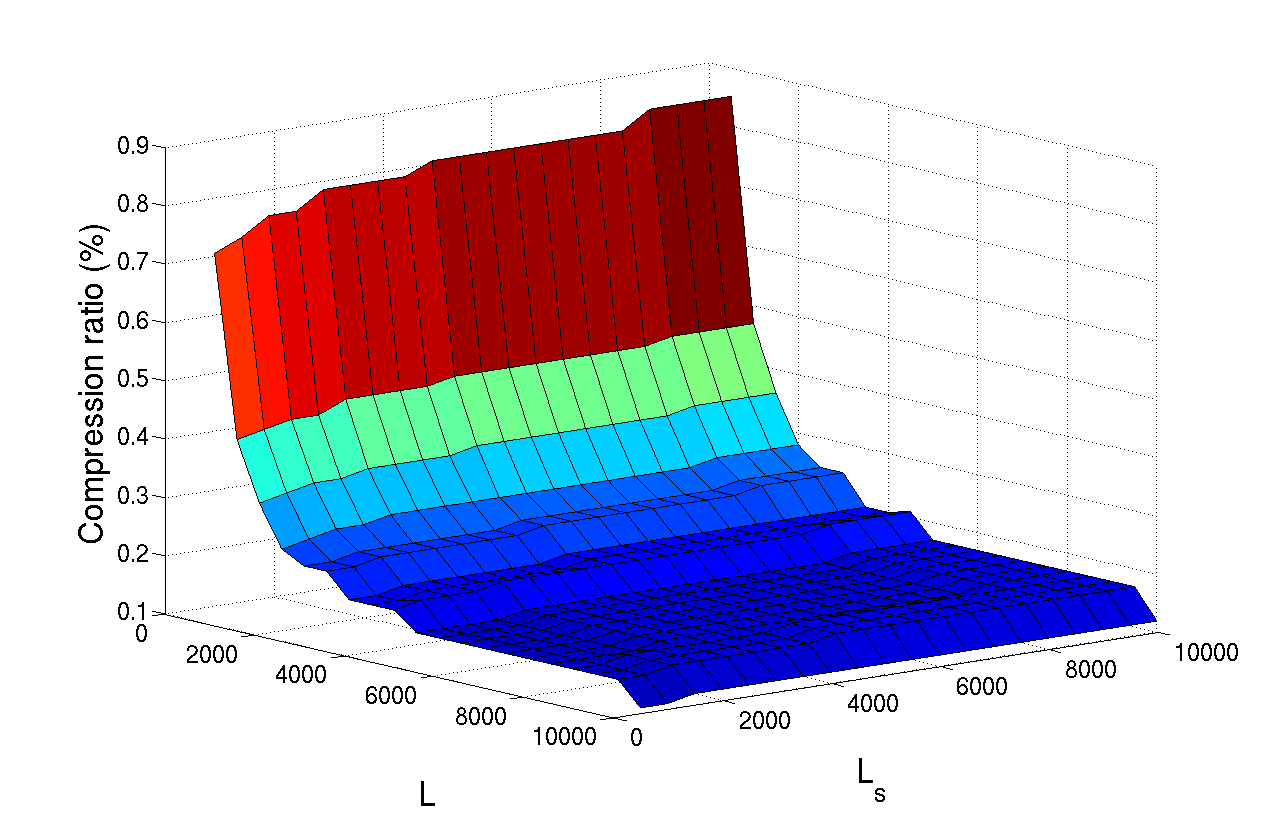
\includegraphics[width=8.5cm]{images/rep_surf.png}
\caption{LZ77 compression ratio in function of $L_s$ and $L_c$.}
\end{figure}
\end{center}

\begin{center}
\begin{figure}[H]
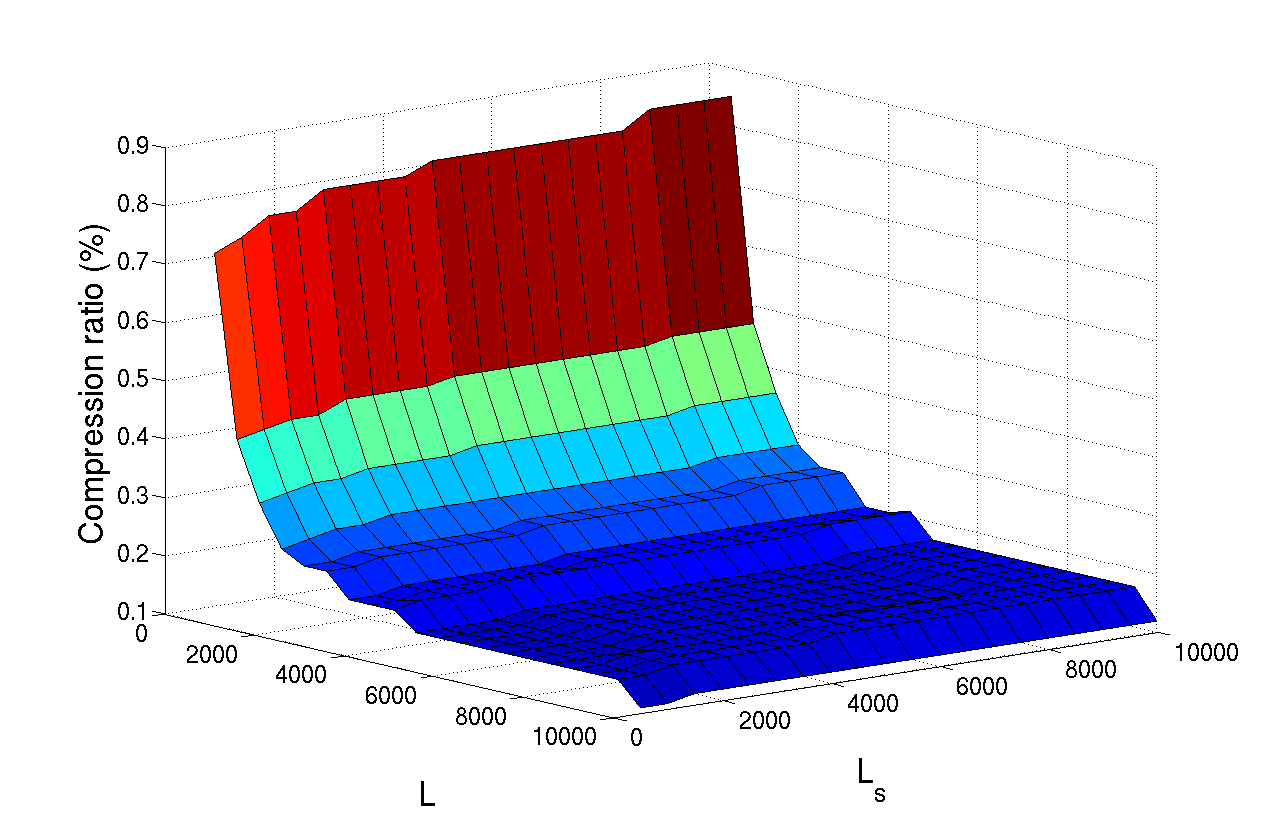
\includegraphics[width=8.5cm]{images/rep_surf.png}
\caption{LZ77 compression ratio in function of $L_s$ and $L_c$.}
\end{figure}
\end{center}

\begin{center}
\begin{figure}[H]
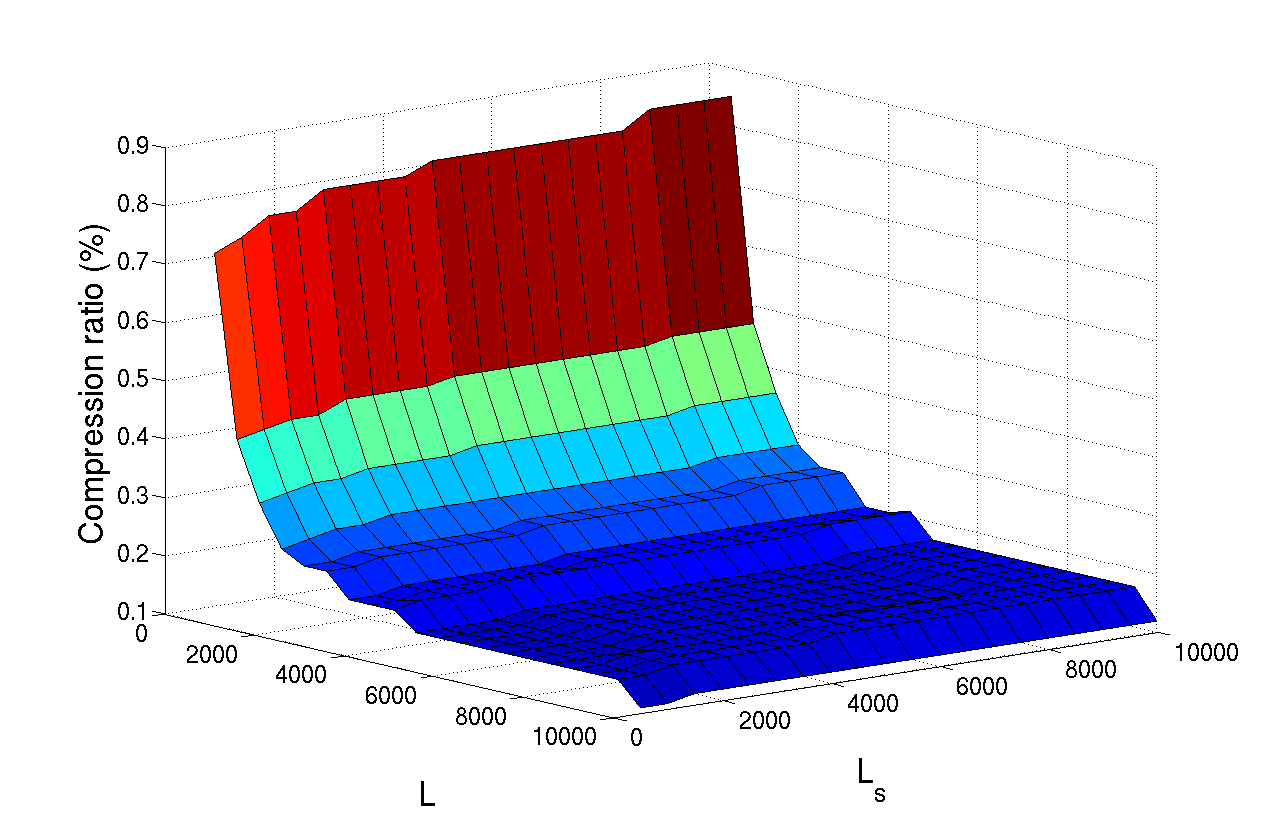
\includegraphics[width=8.5cm]{images/rep_surf.png}
\caption{LZ77 compression ratio in function of $L_s$ and $L_c$.}
\end{figure}
\end{center}

\begin{center}
\begin{figure}[H]
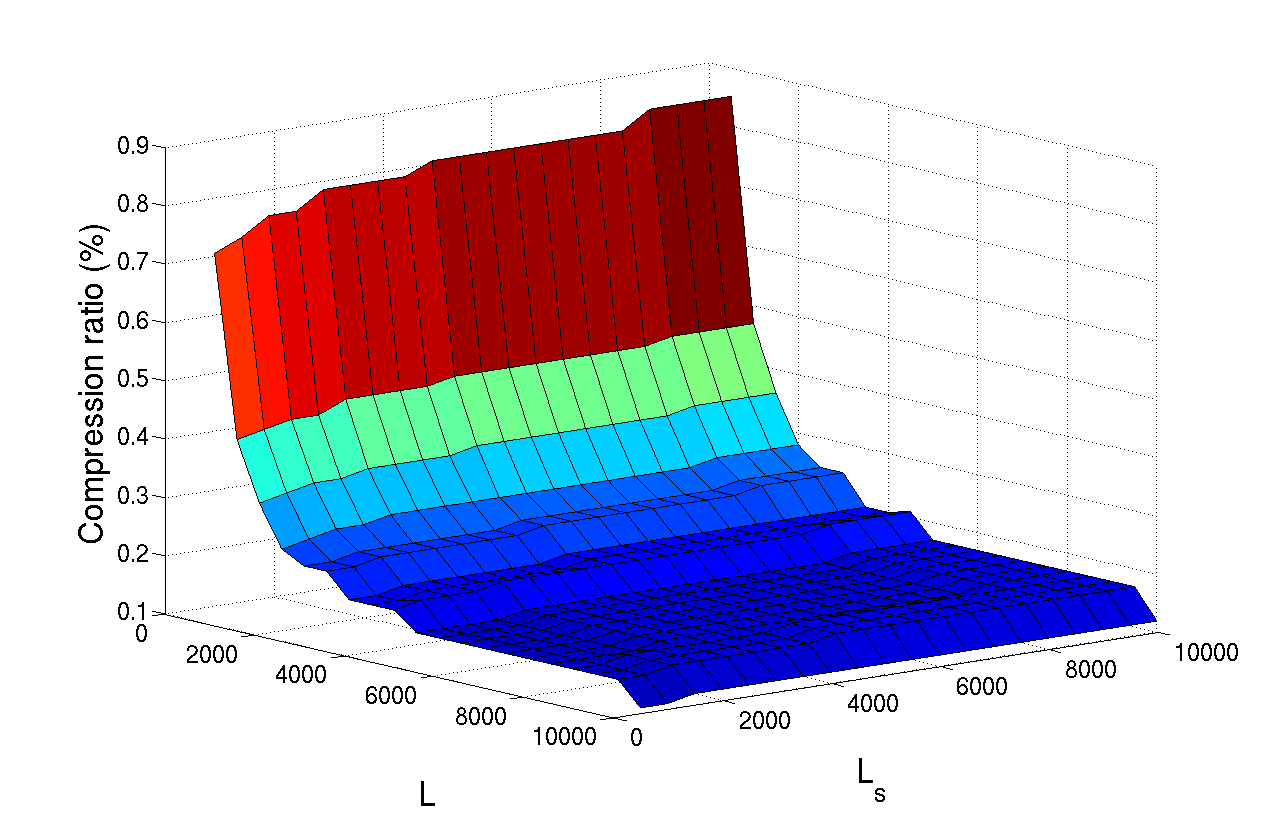
\includegraphics[width=8.5cm]{images/rep_surf.png}
\caption{LZ77 compression ratio in function of $L_s$ and $L_c$.}
\end{figure}
\end{center}

%\begin{center}
%\begin{figure}[H]
%\includegraphics[width=\textwidth]{report_img/snr.eps}
%\caption{Comparison between systems performances.}
%\end{figure}
%\end{center}

%It is easy to see that performances tends to improve with the growing of the \textit{searching window}. We could expect such a result: with shorter windows it is more difficult to find repeated pattern to refer to and, in some cases, we could neither realize that such patterns are present in the message. For a highly redundant input stream a long window allows to encode at the same time much more repetitions; even though the number of bits needed to represent a wide range of values grows with the increasing of the window, this happens with a logarithmic trend, while the amount of space used to encode a sequence byte per byte grows linearly. Clearly the usage of large windows implies a drop of performances from a computational time point of view. 
%In the best compression scenario, we would like to have a \textit{search window} as long as the message itself, but, since this is not suitable for time reason, commercial softwares usually work with block of symbols $32$ Kbyte long with windows of
%
%\subsection{\textit{Searching window} and \textit{coding window} variations}
%The \textit{LZ77} algorithm has, in fact, two parameters we can act to: the lengths of the \textit{searching window} and of the \textit{coding window}. It could be interesting wondering what happens if we stretch both the windows. From the following 2D graphs we can see that the length of the \textit{coding window} has, actually, a low impact on coding performances. The reason is that, for a redundant message, 